\chapter{Digital Filter}
When utilizing a sensor unwanted noise can arise and influence the measurements acquired. By implementing a filter it is possible to attenuate and/or enhance specific frequency components contained in the measurements. When the magnetometer, described in \secref{HardwareChoice}, is active while the vehicle is stationary, the measured angle varies approximately two degrees, see \figref{fig:StationaryMeasurementsMagnato}. The noise affecting the measurements can have a inexpedient effect on the controller which is implemented on the prototype. With ideal circumstances the magnetometer would measure an angle variation of zero degrees. Since this is not the case, implementing a filter to attenuate some of the noise could be a potential solution to get more accuracy.

There is many cons and pros when considering between implementing a analogue or digital filter. But since the signal received from the magnetometer is digitalized, it has been chosen to implement a digital filter.

tail

\section{Filter Considerations}
Header

\subsection{Sampling Frequency}
Header

The transfer function for the plant in the inner loop of the steering model, see \secref{sec:SteeringModel}, is given as:
%
\begin{flalign}
\eq{H(s)}{\frac{K}{(0.03s+1)s}}
\end{flalign}
%
The poles of the system yields 33.3 and 0 \si{\frac{rad}{s}}. When designing a filter it is necessary to consider the placement of the system's dominant pole. in this situation the dominant pole is the pole placed at 33.3 \si{rad/s}. A rule of thumb is to place the cut-off frequency of the filter atleast one decade after the dominant pole, i.e. 333 \si{\frac{rad}{s}}. If the cut-off frequency of the filter is beneath 333 \si{\frac{rad}{s}} it will influence the systems phase-margin, which results in a delay. 

By being aware of this requirement, it is possible to find a sampling frequency which can grant a cut-off frequency above 333 \si{\frac{rad}{s}}. The least required cut-off frequency of 333 \si{\frac{rad}{s}} is calculated to a frequency:
%
\begin{flalign}
\eq{\omega_s}{\frac{333}{2\pi} = 53} \unit{Hz}
\end{flalign}
%
To calculate the least required sampling frequency, the Nyquist-Shannon Sampling Theorem, see \eqref{eq:Nyquistfrequency}, is utilized:
%
\begin{flalign}
\Omega_s &\geq 2 \cdot 53 \leq 106 \unit{Hz}
\end{flalign}
%
The Magnetometer has to be sampled at atleast every 106 \si{Hz}. 

In the specification for the Magnetometer \cite{??}, the sampling rate is given to 75 \si{Hz}. A sampling rate of 106 \si{Hz} was desired, since at this rate it would not effect the system by causing a delay. 

With this in consideration it has been decided to have a sample rate at 66,66 \si{Hz}, i.e. 15 \si{ms}, even though it will cause a delay. The 66,66 \si{Hz} has been chosen instead of the 75 \si{Hz} to have a margin from the maximum sampling rate the sensor can deliver.

\subsection{Frequency Analysis of Measured Data}
Before designing a filter it is necessary to analyse data measured with the magnetometer, to ensure the noise is attenuated and not the wanted signal. The data which is analysed is when the vehicle and the magneto is stationary, this will thereby find the stationary variations on the sensor, the acquired measurements is illustrated in \figref{fig:StationaryMeasurementsMagnato}.

\begin{figure}[H]
  \centering
 	%Trim margins @:   left        bottom       right       top
 	\adjustbox{ trim = {.15\width} {.30\height} {.15\width} {.30\height}, clip }
  {
    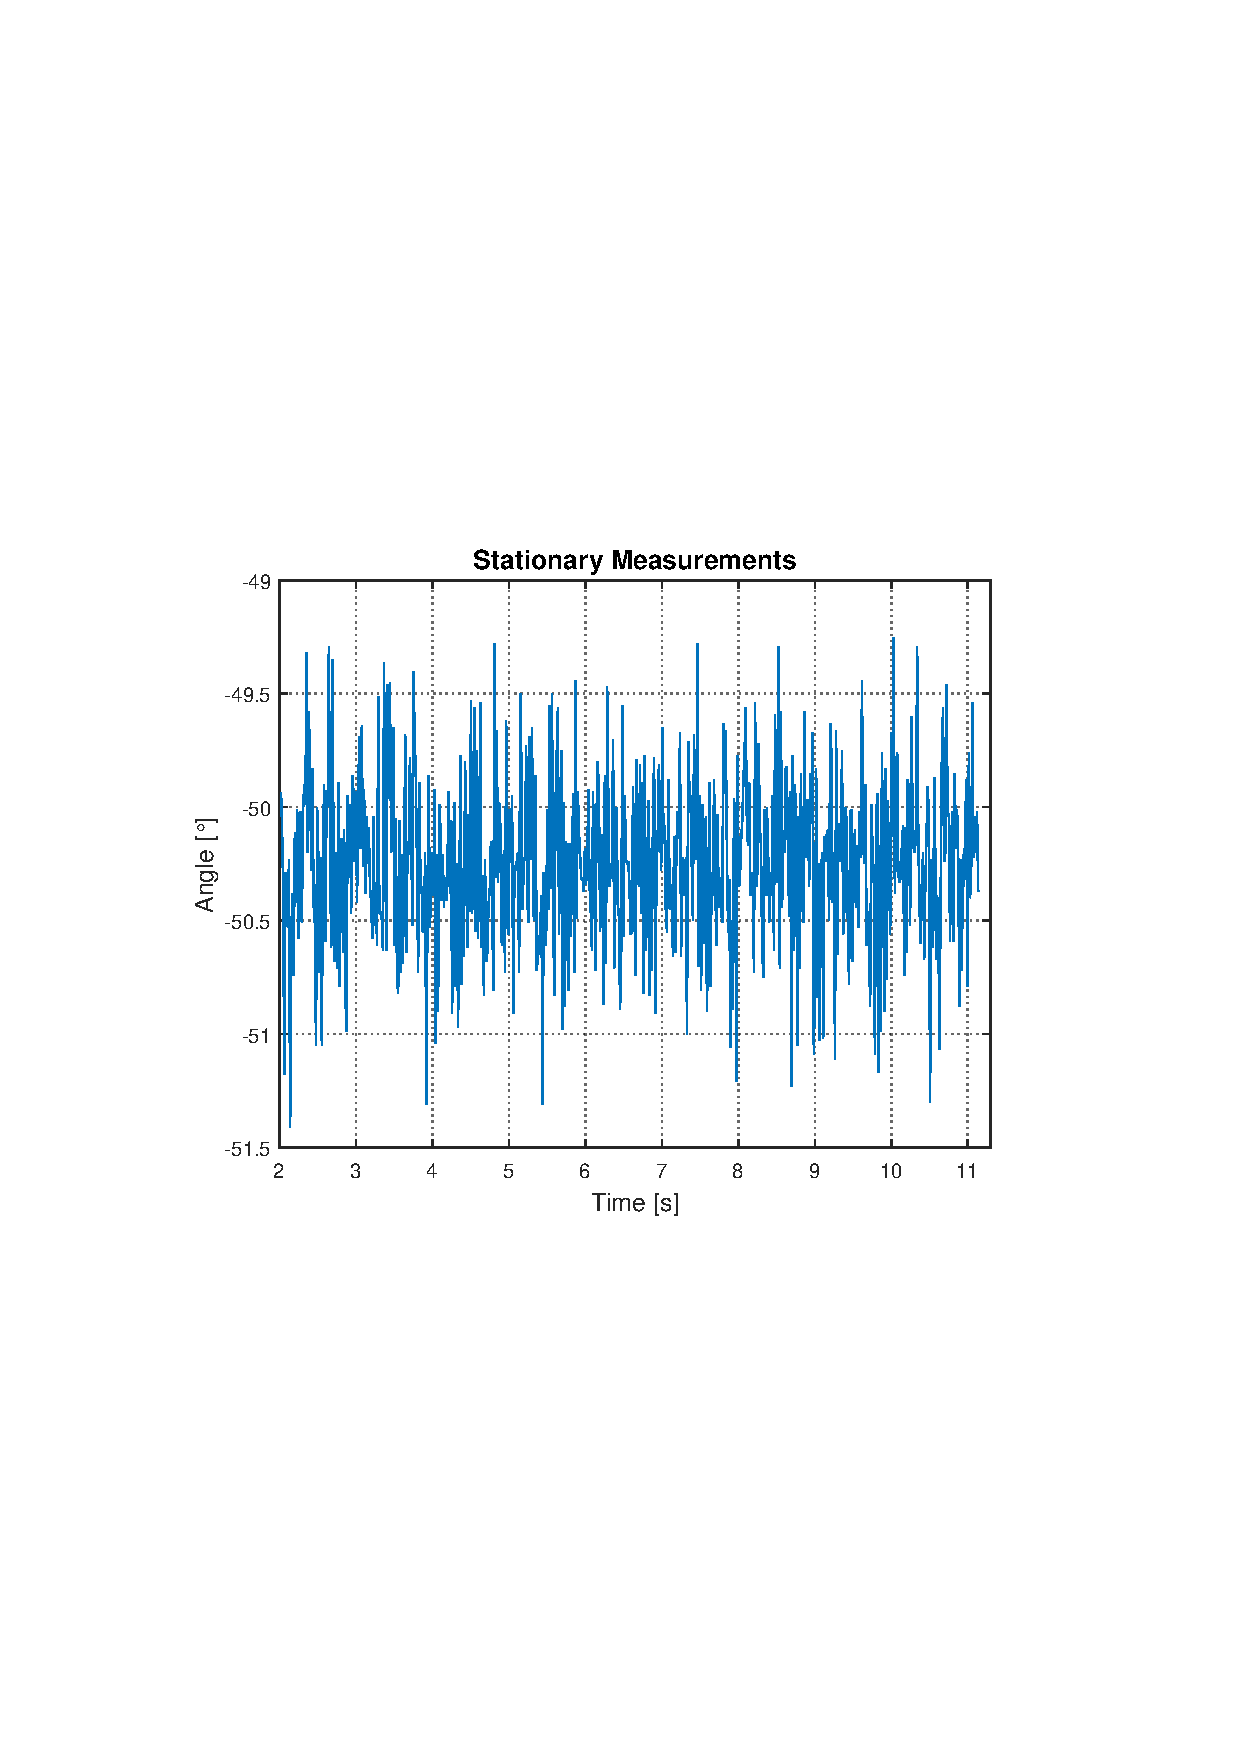
\includegraphics[width=1.1\textwidth]{figures/StationaryMeasurements.pdf}
  }
  \caption{A plot, where the x-axis is time and the y-axis is the angle, of data measured with the magnetometer while the vehicle is stationary.}
  \label{fig:StationaryMeasurementsMagnato}
\end{figure}

From \figref{fig:StationaryMeasurementsMagnato} it can be seen how the angle measured vary with approximately 2 degrees. In the datasheet for the magnetometer it is explained that the sensor has a 1 to 2 degrees accuracy \cite{??}, which is consistent with the measured data. To be able to analyse measured data affected by noise, a FFT is utilized. The FFT makes it possible to see the frequency component contained in the signal, thereby making it possible to find the signal and the noise affecting the signal. A FFT of the measured data is performed and illustrated in \figref{fig:StationaryMeasurementsMagnato}.

\begin{figure}[H]
  \centering
 	%Trim margins @:   left        bottom       right       top
 	\adjustbox{ trim = {.15\width} {.30\height} {.15\width} {.30\height}, clip }
  {
    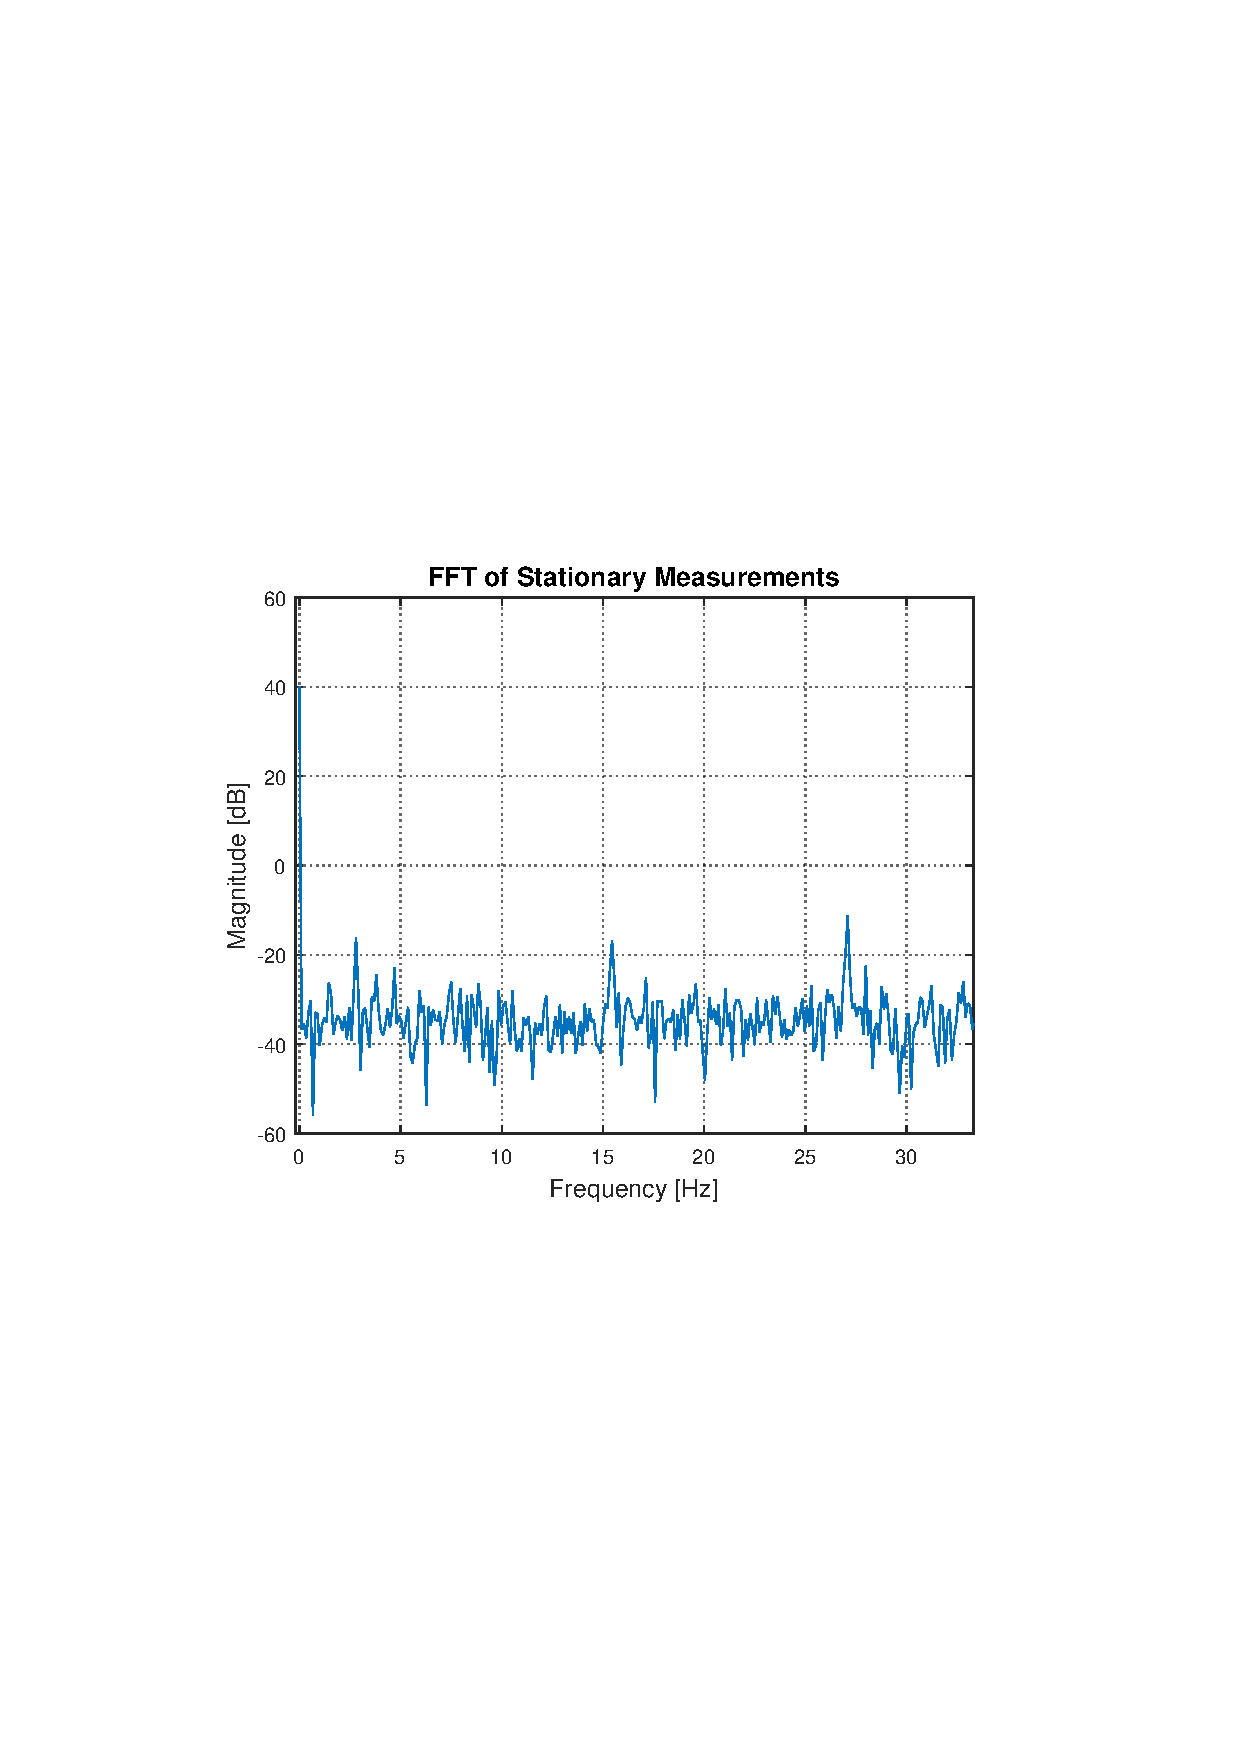
\includegraphics[width=1.1\textwidth]{figures/FFTofStationaryMeasurements.pdf}
  }
  \caption{A FFT of the measured data illustrated in \figref{fig:StationaryMeasurementsMagnato}}
  \label{fig:FFTofStationaryMeasurements}
\end{figure}

The data measured in \figref{fig:StationaryMeasurementsMagnato} is acquired with a sampling frequency of 66.6 \si{Hz}. The Nyquist-Shannon Sampling Theorem says that to find the frequency components contained in a signal you need to have atleast twice the sampling frequency \cite{AVOppenheim}:
%
\begin{flalign}
\Omega_s &\geq 2 \cdot \Omega_N \unit{Hz}
\label{eq:Nyquistfrequency}
\end{flalign}
\hspace{6mm} Where:\\
\begin{tabular}{p{1cm}lll}
& \si{\Omega_s}            	& is the sampling frequency         &\unitWh{Hz} \\
& \si{\Omega_N}				& is the Nyquist frequency			&\unitWh{Hz} \\
\end{tabular}

This is illustrated in \figref{fig:FFTofStationaryMeasurements}, where the frequency components only goes from 0 to 33.3 Hz on the x-axis, which is half the sampling frequency. The y-axis is the magnitude of the frequency component occurring in the signal.

From the FFT performed, seen in \figref{fig:FFTofStationaryMeasurements}, a spike is present at 0 \si{Hz}, this is the DC value, i.e. the offset seen in \figref{fig:StationaryMeasurementsMagnato}. This frequency component is the signal which the filter should not attenuate. The frequency components present after 0 Hz, is the noise from the sensor. 

Some consideration has to be made for the filter requirements, to ensure that the filter is not influencing the system and the desired frequency needlessly.

\subsection{Filter Type}
Data from the filter has been examined, it is thereby possible to examine which filter would be suitable for fulfilling the predetermined requirements. It should do this without influencing the DC-value and the system needlessly.

\begin{figure}[H]
	\centering
	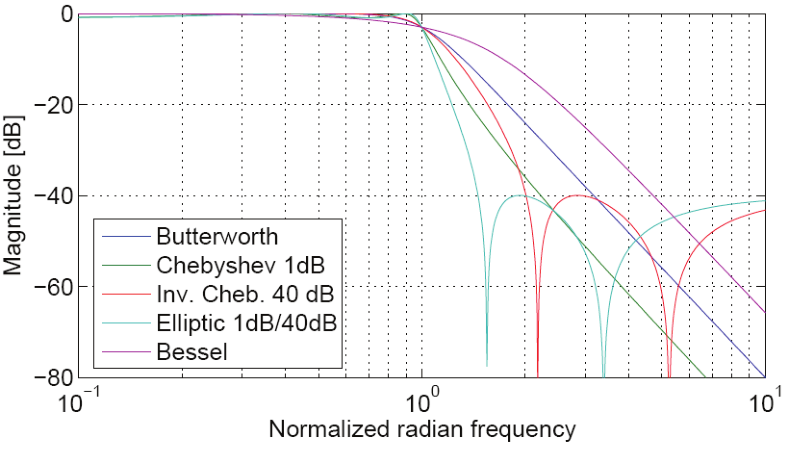
\includegraphics[scale=1]{figures/Filtertypes1.pdf}
	\caption{Frequency response for various filter types}
	\label{fig:Filtertype1}
\end{figure}

The disadvantages of a Elliptic filter is that it has both ripples in the pass- and stopband. additionally, it has a high group delay both before and at the cutoff frequency, this can be seen in \figref{fig:groupdelay}. The advantage of a Elliptic filter is that is has the sharpest cut-off frequency of the filters illustrated in \figref{fig:Filtertype1}.

The Chebyshev filter only has ripples in the passband, and a sharp cut-off frequency, but still has a high group delay before and at the cut-off frequency. The inverse Chebyshev only has ripples in the stopband, but does not have as sharp cut-off frequency as the Chebyshev and the Elliptic filter. Compared to the two former filter it has a lot less group delay before and after the cut-off frequency.

The Bessel filter has the lowest group delay before and at the cut-off frequency, see \figref{fig:groupdelay}. additionally, it does not have any ripples, neither in pass- or stopband. The disadvantage of the filter is it has the least sharpest cut-off frequency of the filters illustrated in \figref{fig:Filtertype1}.

The Butterworth filter has a sharper cut-off frequency compared to the Bessel filter and as the Bessel filter it does not have any ripples neither in the pass- or stopband. Furhtermore, the Butterworth filter has the second lowest group delay at the cut-off frequency compared to the other filters illustrated in \figref{fig:groupdelay}. 

\begin{figure}[H]
	\centering
	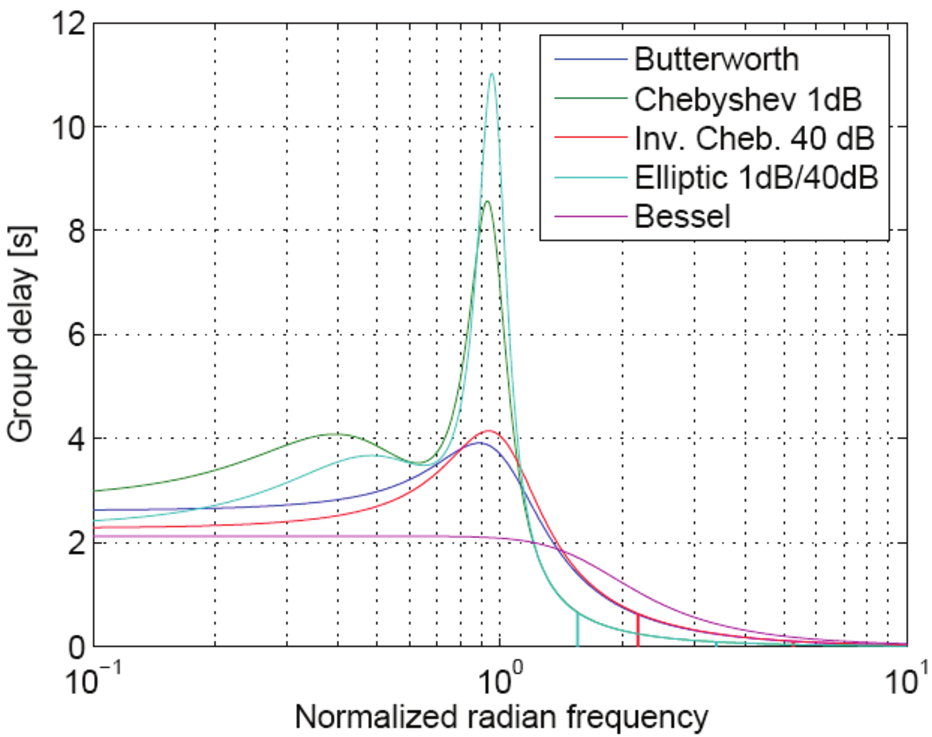
\includegraphics[scale=0.7]{figures/Filtertypes2.pdf}
	\caption{Frequency response illustrating group delay for various filter types}
	\label{fig:groupdelay}
\end{figure}

Because of the above-mentioned descriptions of the filters, a Butterworth filter has been selected for filtering the measured data. The Butterworth does not have any ripples in the passband which could influence the DC-value, seen in \figref{fig:FFTofStationaryMeasurements}, and compared to the other described filters, the Butterworth has a small group delay.

Considerations for the filter has been made, and it is thereby possible to specify the requirements for the filter.

\section{Filter Requirements} \label{sec:FilterRequirements}
Header





\section{Design}

\subsection{Bilinear Transform vs. Impulse Invariance transformation}
There is different methods for transferring a continuous-time filter to a discrete-time filter, the two most common transformation methods is examined. The first method which is examined is the impulse variance transformation.

When utilizing the impulse invariance transformation a discrete filter is generated by sampling a impulse response of a continuous analogue prototype filter. The impulse response of the discrete-time filter is proportional to the impulse response of the continuous-time filter with equally spaced samples, i.e.  making the discrete-filter from a sampled continuous-time prototype filter, see \eqref{impulseresponsepropotional}, \cite{AVOppenheim}.
%
\begin{flalign}
h[nT] &= h[n] = T \cdot h(t) \big\vert_{t=nT}&
\label{impulseresponsepropotional}
\end{flalign}
%
This makes it a linear mapping, \si{\omega = \Omega \cdot T_d} for each pole in the analogue filter's transfer function on the s-plane to a pole on the z-plane. 

The main issue when utilizing the impulse variance method is that the sampling rate needs to be relatively high compared to the filter's bandwidth, to not cause aliasing \cite{LyonsR.G}. In the frequency response, seen in \figref{fig:ImpulseVariantFrequencyResponse}, it can be seen that the response of a 6th-order Butterworth filter transformed by impulse invariance, has a frequency response which is larger than from 0 to \si{pi}, hence causing aliasing.

\begin{figure}[H]
	\centering
	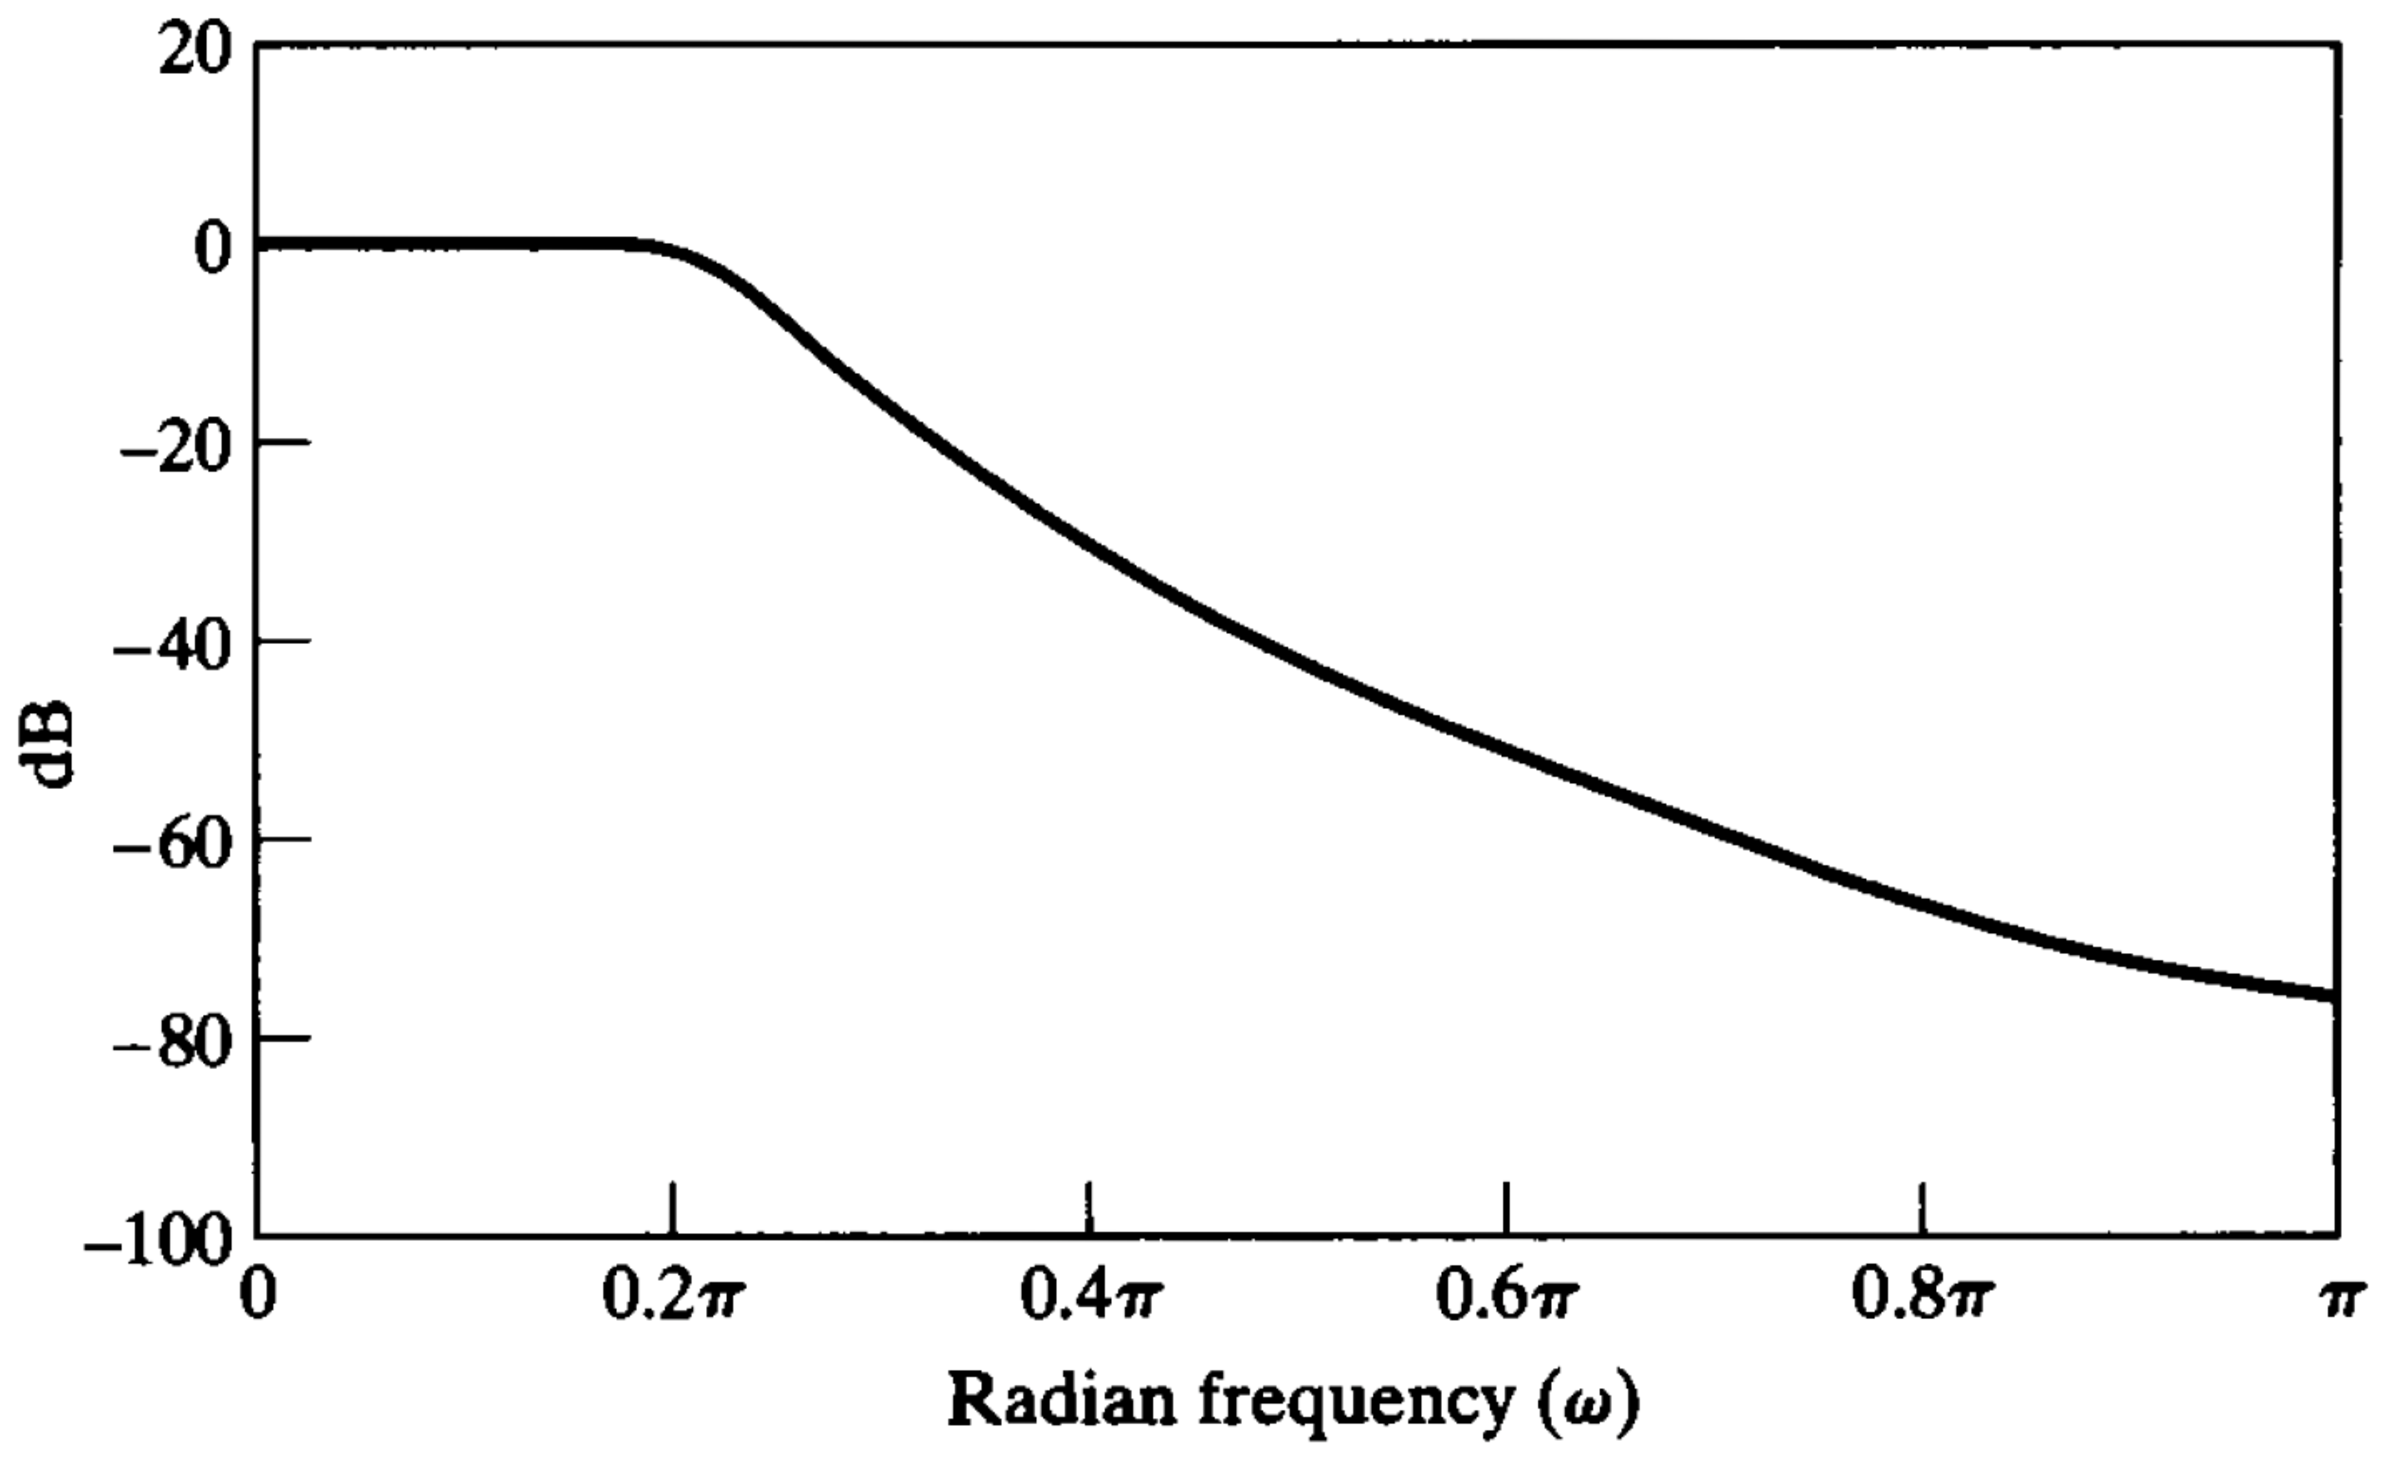
\includegraphics[scale=0.2]{figures/BilinearFrequencyResponse.pdf}
	\caption{A frequency response of a transformed impulse variance 6th order Butterworth filter \cite{AVOppenheim}.}
	\label{fig:ImpulseVariantFrequencyResponse}
\end{figure}

The Bilinear transform also utilize a analogue prototype filter to convert from s-domain to z-domain, when designing a digital filter. This transformation type is not a linear transformation from the s-domain to the z-domain as it is with the impulse variance method. Instead it is a non-linear transformation which is mapping poles from \si{-\infty < \Omega < \infty} in the s-domain to \si{-\pi < \omega < \pi} in the z-domain \cite{OlesSlides}. This yields a relationship between the continuous-time frequencies to the discrete-time frequencies called pre-warping.
%
\begin{flalign}
\omega &= 2 \cdot \arctan(\frac{\Omega \cdot T_d}{2}) \wedge \Omega = \frac{2}{T_d} \cdot \tan(\frac{\omega}{2}) &
\label{eq:bilinearprewarp}
\end{flalign}
%
A frequency response of the same filter, as the frequency response for the impulse invariance, is illustrated in \figref{fig:BilinearFrequencyResponse}. The bilinear transform avoids aliasing problems because it maps the s-planes imaginary axis onto the z-planes unit circle \cite{AVOppenheim}, which can be seen in \figref{fig:S-planeVsZ-plane}.
%
\begin{figure}[H]
	\centering
	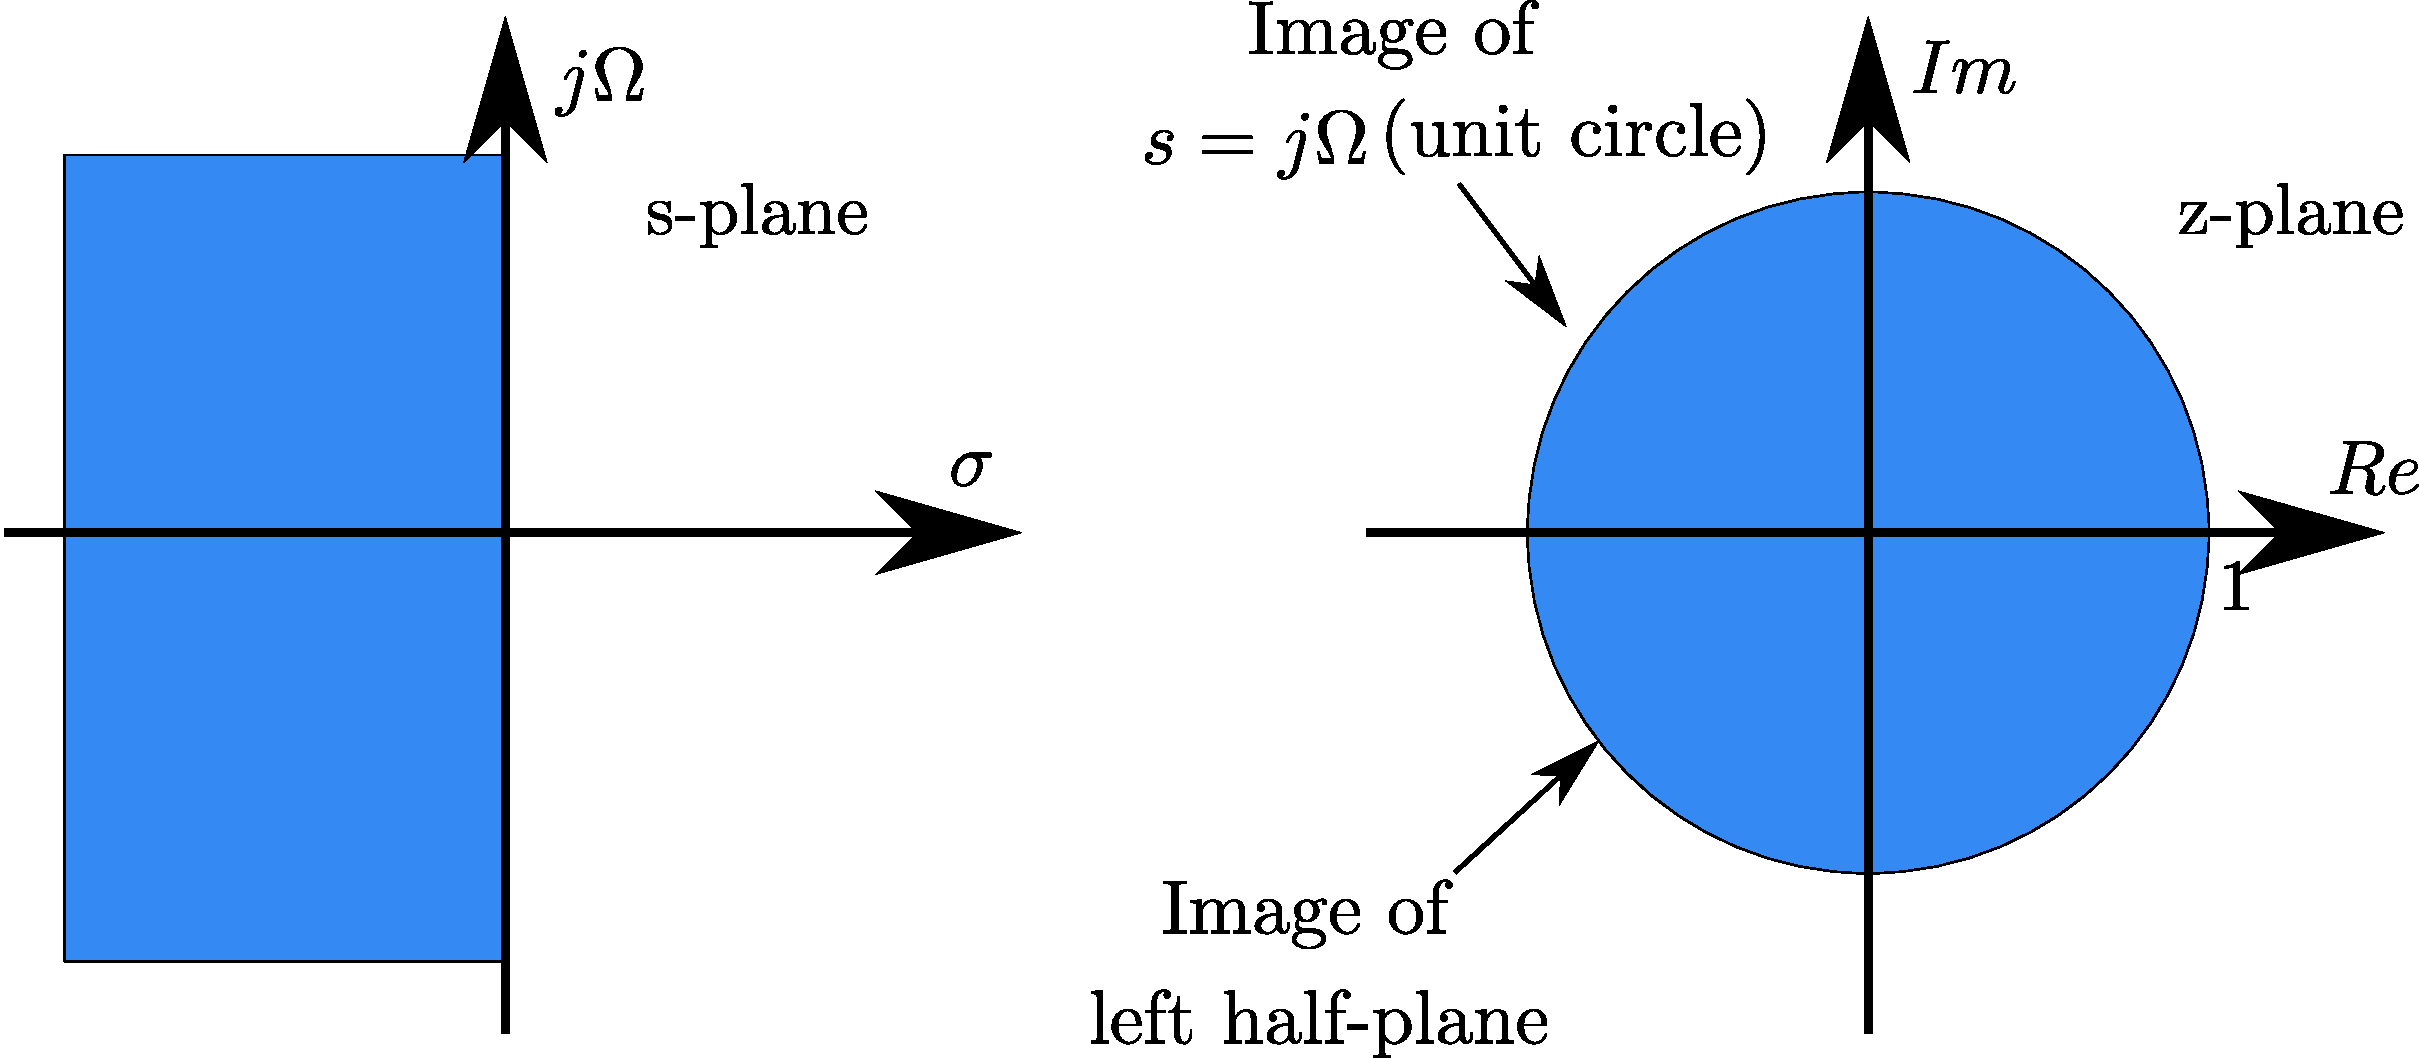
\includegraphics[scale=0.3]{figures/SplaneVsZplane.pdf}
	\caption{s-domain and z-domain \cite{AVOppenheim}.}
	\label{fig:S-planeVsZ-plane}
\end{figure}
%
From \figref{fig:BilinearFrequencyResponse} it can be seen that the frequency response does not exceed the limit from 0 to \si{pi}, hence not causing a aliasing problem \cite{AVOppenheim}.

\begin{figure}[H]
	\centering
	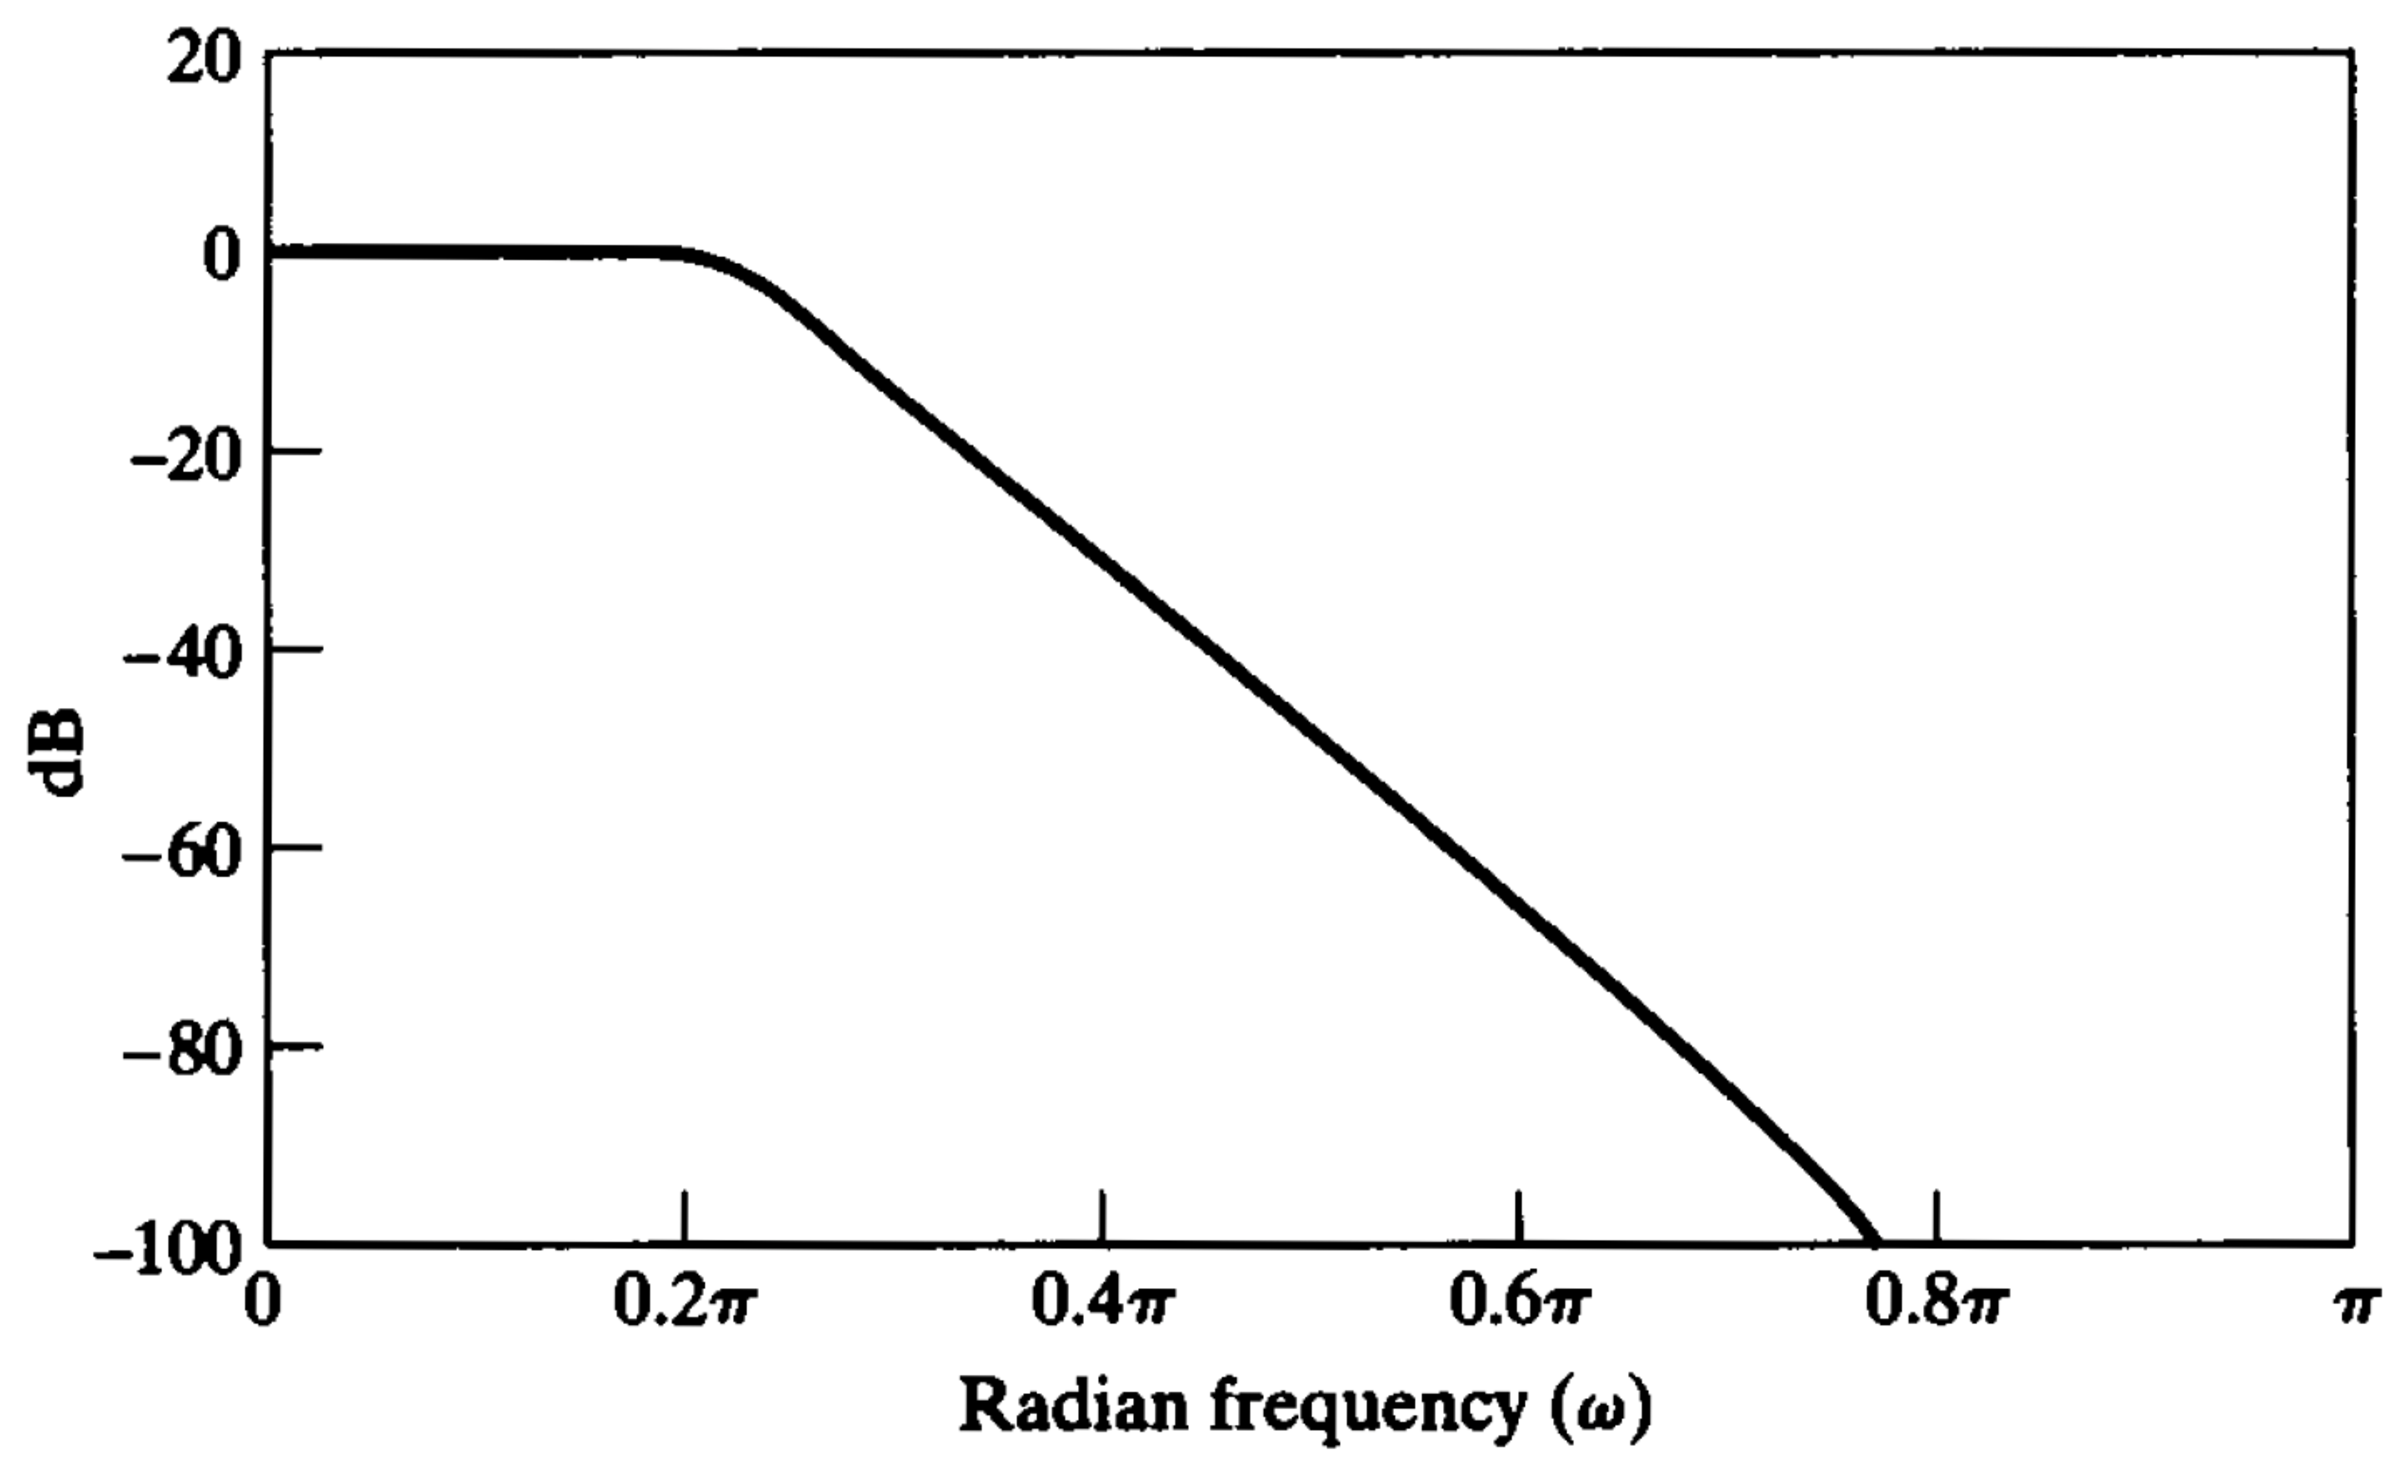
\includegraphics[scale=0.2]{figures/ImpulseVariantFrequencyResponse.pdf}
	\caption{A frequency response of a transformed bilinear transform 6th order Butterworth filter \cite{AVOppenheim}.}
	\label{fig:BilinearFrequencyResponse}
\end{figure}

It has been chosen to use the bilinear transformation when designing the filter. This is mainly do to the issue with aliasing that occurs when utilizing impulse variance transform which does not happen when utilizing bilinear transform.

\subsection{Designing a low-pass Butterworth filter using the bilinear transform}
When utilizing bilinear transform it is necessary to frequency warp the passband frequency and the stopband frequency, from \secref{sec:FilterRequirements}. This is done by utilizing the relationship between the discrete-time frequencies in the z-domain to the continuous-time frequencies in the s-domain illustrated in \eqref{eq:bilinearprewarp}. 
%
\begin{flalign}
\Omega_p &= \frac{2}{0.030} \cdot \tan(\frac{0.5 \pi}{2}) = 66.7 \quad \wedge \quad \Omega_s = \frac{2}{0.030} \cdot \tan(\frac{0.85 \pi}{2}) = 277.69 \unit{Hz}
\end{flalign}
\hspace{6mm} Where:\\
\begin{tabular}{p{1cm}lll}
& \si{\Omega_p} & is the passband frequency in continuous time &\unitWh{Hz} \\
& \si{\Omega_s}	& is the stopband frequency in continuous time &\unitWh{Hz} \\
\end{tabular}

By utilizing the magnitude squared function for a Butterworth filter, it is possible to find the cut-off frequency:
%
\begin{flalign}
\eq{|H(e^{j\omega}|^2}{\frac{1}{1+(\frac{\Omega}{\Omega_c})^{2N}}}
\end{flalign}
\hspace{6mm} Where:\\
\begin{tabular}{p{1cm}lll}
& \si{\Omega}       & is the pre-warped frequencies  &\unitWh{Hz} \\
& \si{\Omega_C}		& is the cut-off frequency &\unitWh{Hz} \\
& \si{|H(e^{j\omega}|} & is the attenuation requirements set for the different bands from \secref{sec:FilterRequirements} &\unitWh{dB}
\end{tabular}
%
\begin{flalign}
\eq{0.89125^2}{\frac{1}{1+(\frac{66.7}{\Omega_C})^{2 \cdot 4}} = 78.933} \unit{Hz}
\end{flalign}
%
The cut-off frequency is calculated to 78.933 \si{Hz}. When the order is known it is possible to utilize the following equation for finding the poles for a Butterworth filter.
%
\begin{flalign}
\eq{P_k}{\Omega_c \cdot e^{j(\frac{2 \cdot k -1}{2 \cdot N} \cdot \pi + \frac{\pi}{2})}}
\end{flalign}
%
Where k equal 1,2 \si{\dotsc N}.

Since it would desirable to have a stable system, the poles should only be located on the left side of the y-axis in the s-plane.
%
\begin{flalign}
\eq{P_1}{\Omega_c \cdot e^{j \cdot \frac{5}{8} \pi}} \\
\eq{P_2}{\Omega_c \cdot e^{j \cdot \frac{7}{8} \pi}} \\
\eq{P_3}{\Omega_c \cdot e^{j \cdot \frac{9}{8} \pi}} \\
\eq{P_4}{\Omega_c \cdot e^{j \cdot \frac{11}{8} \pi}}
\end{flalign}
%
The general transfer function for a Butterworth filter is defined as:
%
\begin{flalign}
\eq{H(s)}{\frac{G_o}{\prod\limits_{k = 1}^N (s-P_k)}}
\end{flalign}
\hspace{6mm} Where:\\
\begin{tabular}{p{1cm}lll}
& \si{G_o}       & is the gain of the filter  &\unitWh{\cdot} \\
\end{tabular}

\todo{something about gain}

\begin{flalign}
\eq{H(s)}{\frac{\Omega_c^4}{(s-\Omega_ce^{j\cdot \frac{5}{8} \cdot \pi})(s-\Omega_ce^{j\cdot \frac{7}{8} \cdot \pi})(s-\Omega_ce^{j\cdot \frac{9}{8} \cdot \pi})(s-\Omega_ce^{j\cdot \frac{11}{8} \cdot \pi})}}
\end{flalign}

It can be seen from the placement of the poles, that there is two complex pole-pair. By utilizing the rule \si{s = s*}, it is possible to change the transfer function.
%
\begin{flalign}
\eq{H(s)}{\frac{\Omega_c^4}{(s-\Omega_ce^{j\cdot \frac{5}{8} \cdot \pi})(s-\Omega_ce^{j\cdot \frac{7}{8} \cdot \pi})(s-\Omega_ce^{-j\cdot \frac{7}{8} \cdot \pi})(s-\Omega_ce^{-j\cdot \frac{5}{8} \cdot \pi})}}
\end{flalign}
%
Transforming the complex poles to standard form:
%
\begin{flalign}
\eq{H(s)}{\frac{\Omega_c^4}{(s^2 + 2 \cdot \cos{(\frac{7}{8} \cdot \pi)} \cdot \Omega_c \cdot s + \Omega_c^2)(s^2 + 2 \cdot \cos{(\frac{5}{8} \cdot \pi)} \cdot \Omega_c \cdot s + \Omega_c^2)}}
\end{flalign}

\begin{figure}[H]
  \centering
 	%Trim margins @:   left        bottom       right       top
 	\adjustbox{ trim = {.15\width} {.30\height} {.15\width} {.30\height}, clip }
  {
    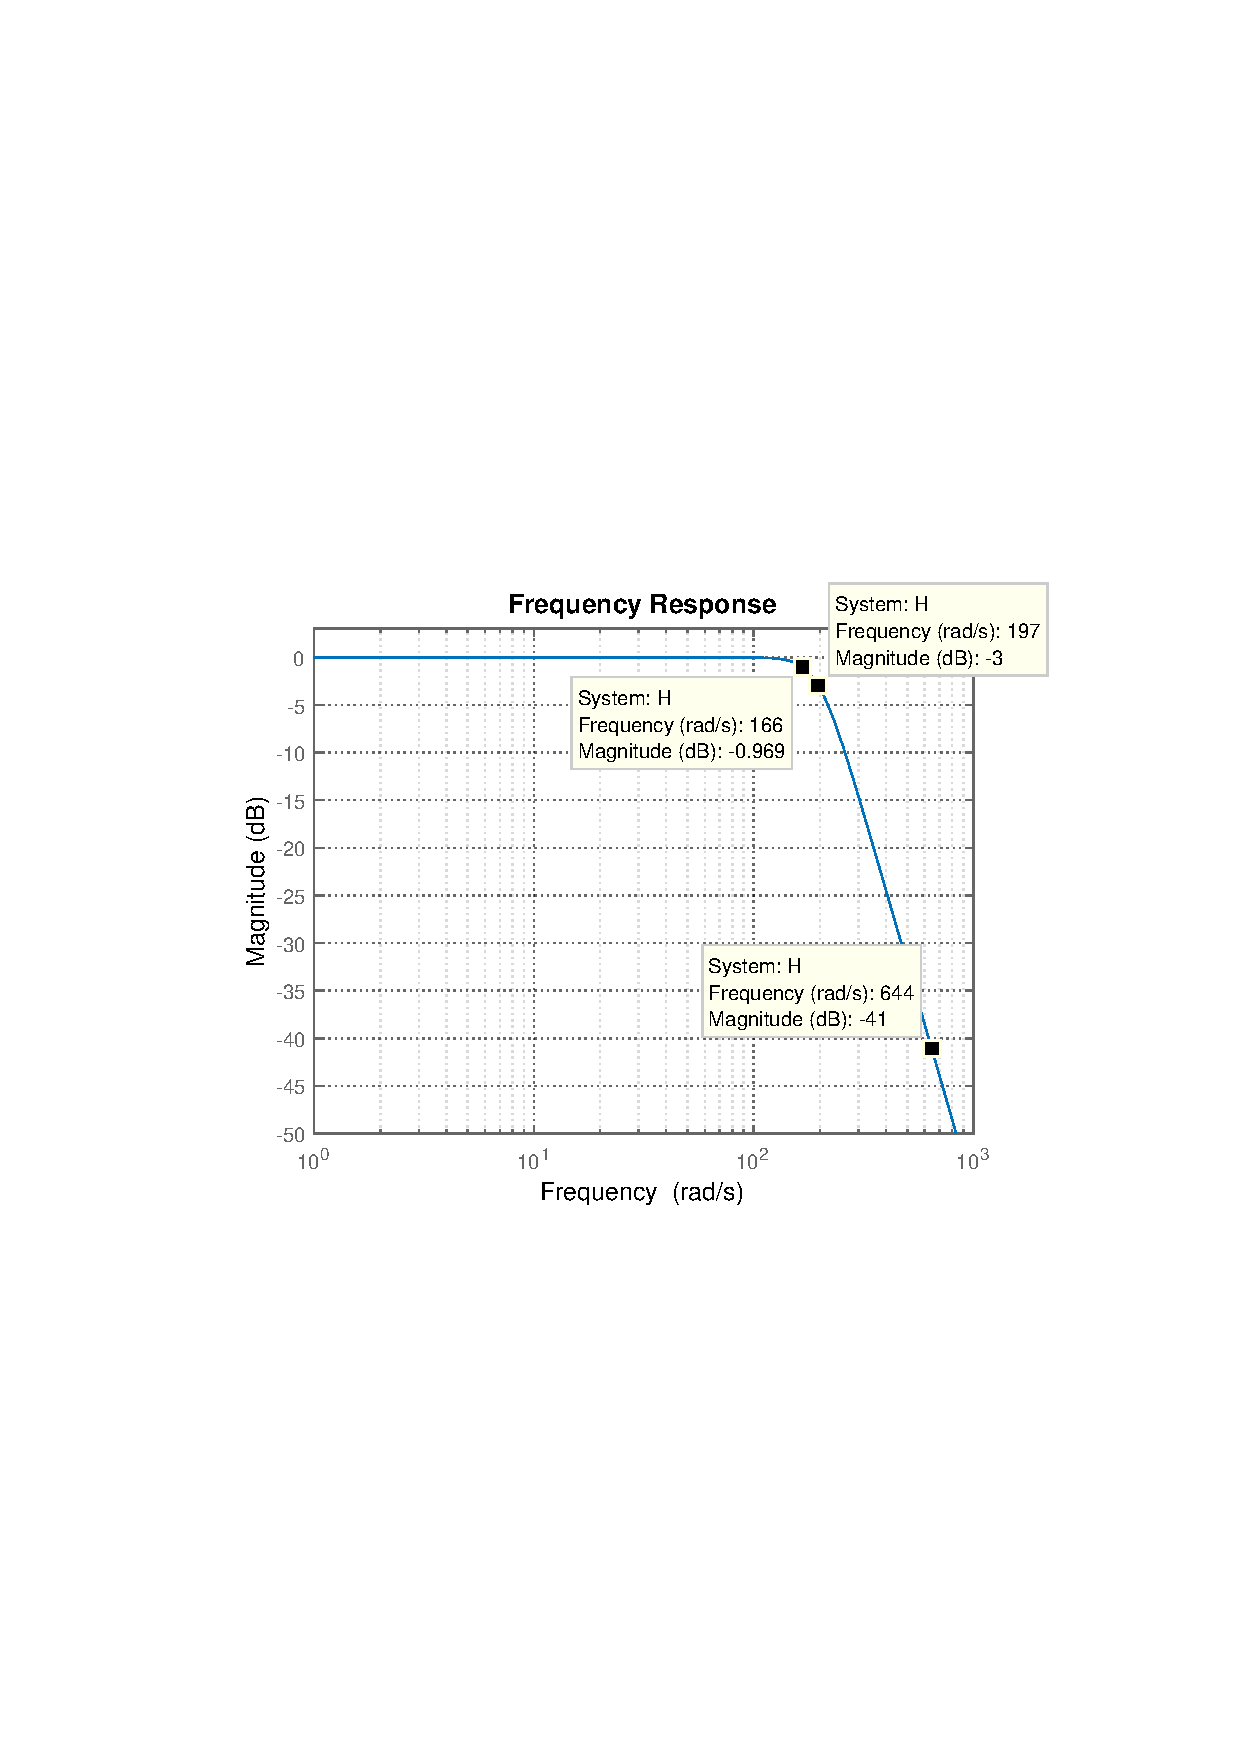
\includegraphics[width=1.1\textwidth]{figures/ContinusFilterResponse.pdf}
  }
  \caption{A FFT of the measured data illustrated in \figref{fig:StationaryMeasurementsMagnato}}
  \label{fig:Continuoustimebodeplot}
\end{figure}

The next step would be to transfer the continuous-time Butterworth filter to the z-domain.

\subsection{Transforming the filter to Z-domain}

\begin{flalign}
\eq{s}{\frac{2}{T_d}(\frac{1-z^{-1}}{1+z^{-1}})}
\end{flalign}

\begin{figure}[H]
  \centering
 	%Trim margins @:   left        bottom       right       top
 	\adjustbox{ trim = {.15\width} {.30\height} {.15\width} {.30\height}, clip }
  {
    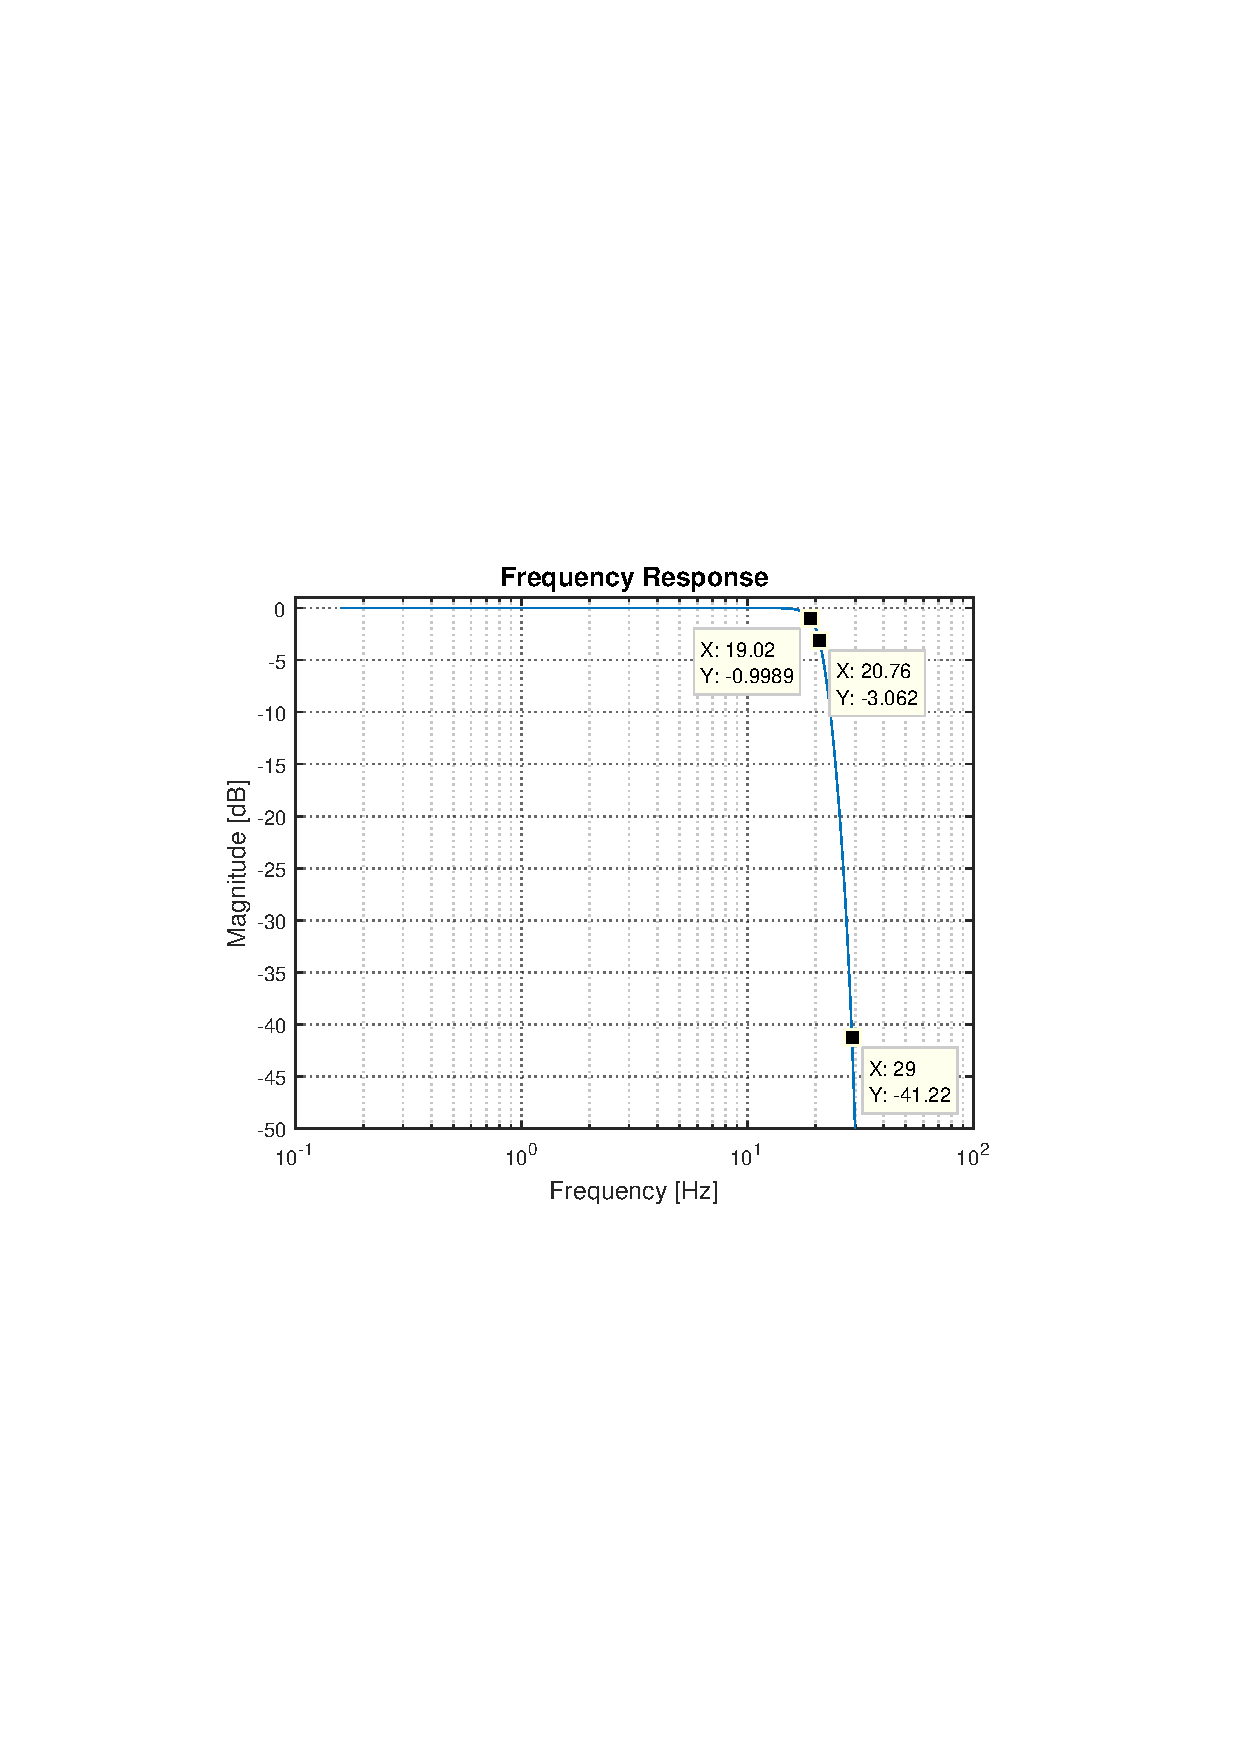
\includegraphics[width=1.1\textwidth]{figures/DiscreteFrequencyResponse.pdf}
  }
  \caption{A FFT of the measured data illustrated in \figref{fig:StationaryMeasurementsMagnato}}
  \label{fig:discretetimebodeplot}
\end{figure}



Standard formula:

\begin{flalign}
H(z) &= \frac{B(z)}{A(z)} = \frac{b_0 + b_1z^-1 + b_2z^-2 + \dotsc + b_Nz^{-N}}{1 + a_1z^-1 + a_2z^-2 + \dotsc + a_Mz^{-M}}
\end{flalign}

\begin{flalign}
H(z) &= \frac{B(z)}{A(z)} = \frac{0.1326 + 0.5305z^{-1} + 0.7957z^{-2} + 0.5305z^{-3} + 0.1326z^{-4}}{1 + 0.4515z^{-1} + 0.5505z^{-2} + 0.09825z^{-3} + 0.02167z^{-4}}
\end{flalign}

\section{Implementation}


\lstset{language=Matlab, caption={Code Implementation in Matlab}, label=lst:FilterMatlabImplementation}
\begin{lstlisting}
for i = 1:707

  BUF0 = input(i) - (a1*BUF1 + a2*BUF2 + a3*BUF3 + a4*BUF4)
	
  output(i) = BUF0*b0 + b1*BUF1 + b2*BUF2 + b3*BUF3 + b4*BUF4
    	
  BUF4 = BUF3
  BUF3 = BUF2
  BUF2 = BUF1
  BUF1 = BUF0
    
 end
\end{lstlisting}

\section{Results}

\begin{figure}[H]
  \centering
 	%Trim margins @:   left        bottom       right       top
 	\adjustbox{ trim = {.15\width} {.30\height} {.15\width} {.30\height}, clip }
  {
    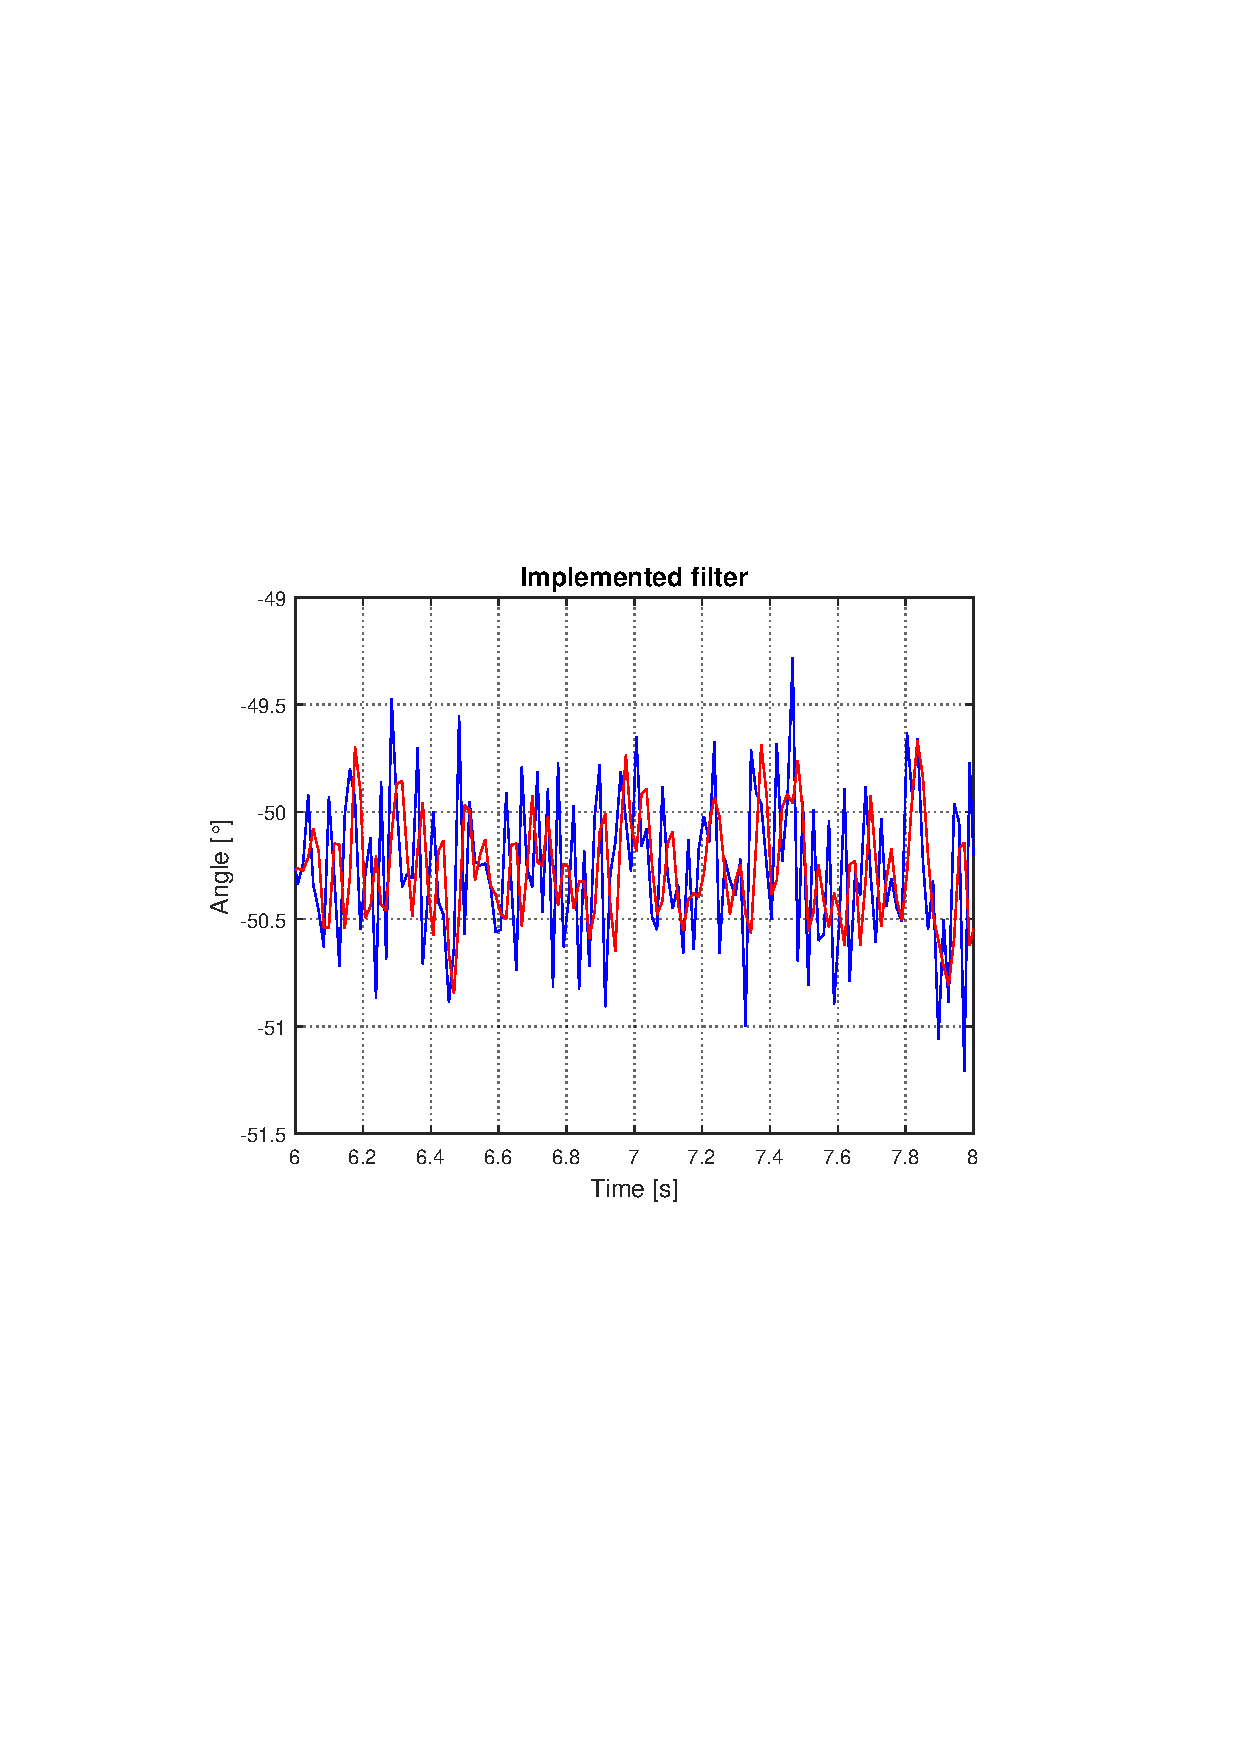
\includegraphics[width=1.1\textwidth]{figures/ImplementedFilter.pdf}
  }
  \caption{A FFT of the measured data illustrated in \figref{fig:StationaryMeasurementsMagnato}}
  \label{fig:discretetimebodeplot}
\end{figure}
